\documentclass[english,floatsintext,man]{apa6}

\usepackage{amssymb,amsmath}
\usepackage{ifxetex,ifluatex}
\usepackage{fixltx2e} % provides \textsubscript
\ifnum 0\ifxetex 1\fi\ifluatex 1\fi=0 % if pdftex
  \usepackage[T1]{fontenc}
  \usepackage[utf8]{inputenc}
\else % if luatex or xelatex
  \ifxetex
    \usepackage{mathspec}
    \usepackage{xltxtra,xunicode}
  \else
    \usepackage{fontspec}
  \fi
  \defaultfontfeatures{Mapping=tex-text,Scale=MatchLowercase}
  \newcommand{\euro}{€}
\fi
% use upquote if available, for straight quotes in verbatim environments
\IfFileExists{upquote.sty}{\usepackage{upquote}}{}
% use microtype if available
\IfFileExists{microtype.sty}{\usepackage{microtype}}{}

% Table formatting
\usepackage{longtable, booktabs}
\usepackage{lscape}
% \usepackage[counterclockwise]{rotating}   % Landscape page setup for large tables
\usepackage{multirow}		% Table styling
\usepackage{tabularx}		% Control Column width
\usepackage[flushleft]{threeparttable}	% Allows for three part tables with a specified notes section
\usepackage{threeparttablex}            % Lets threeparttable work with longtable

% Create new environments so endfloat can handle them
% \newenvironment{ltable}
%   {\begin{landscape}\begin{center}\begin{threeparttable}}
%   {\end{threeparttable}\end{center}\end{landscape}}

\newenvironment{lltable}
  {\begin{landscape}\begin{center}\begin{ThreePartTable}}
  {\end{ThreePartTable}\end{center}\end{landscape}}




% The following enables adjusting longtable caption width to table width
% Solution found at http://golatex.de/longtable-mit-caption-so-breit-wie-die-tabelle-t15767.html
\makeatletter
\newcommand\LastLTentrywidth{1em}
\newlength\longtablewidth
\setlength{\longtablewidth}{1in}
\newcommand\getlongtablewidth{%
 \begingroup
  \ifcsname LT@\roman{LT@tables}\endcsname
  \global\longtablewidth=0pt
  \renewcommand\LT@entry[2]{\global\advance\longtablewidth by ##2\relax\gdef\LastLTentrywidth{##2}}%
  \@nameuse{LT@\roman{LT@tables}}%
  \fi
\endgroup}


  \usepackage{graphicx}
  \makeatletter
  \def\maxwidth{\ifdim\Gin@nat@width>\linewidth\linewidth\else\Gin@nat@width\fi}
  \def\maxheight{\ifdim\Gin@nat@height>\textheight\textheight\else\Gin@nat@height\fi}
  \makeatother
  % Scale images if necessary, so that they will not overflow the page
  % margins by default, and it is still possible to overwrite the defaults
  % using explicit options in \includegraphics[width, height, ...]{}
  \setkeys{Gin}{width=\maxwidth,height=\maxheight,keepaspectratio}
\ifxetex
  \usepackage[setpagesize=false, % page size defined by xetex
              unicode=false, % unicode breaks when used with xetex
              xetex]{hyperref}
\else
  \usepackage[unicode=true]{hyperref}
\fi
\hypersetup{breaklinks=true,
            pdfauthor={},
            pdftitle={A Quantitative Synthesis of Early Language Acquisition Using Meta-Analysis},
            colorlinks=true,
            citecolor=blue,
            urlcolor=blue,
            linkcolor=black,
            pdfborder={0 0 0}}
\urlstyle{same}  % don't use monospace font for urls

\setlength{\parindent}{0pt}
%\setlength{\parskip}{0pt plus 0pt minus 0pt}

\setlength{\emergencystretch}{3em}  % prevent overfull lines

\ifxetex
  \usepackage{polyglossia}
  \setmainlanguage{}
\else
  \usepackage[english]{babel}
\fi

% Manuscript styling
\captionsetup{font=singlespacing,justification=justified}
\usepackage{csquotes}
\usepackage{upgreek}



\usepackage{tikz} % Variable definition to generate author note

% fix for \tightlist problem in pandoc 1.14
\providecommand{\tightlist}{%
  \setlength{\itemsep}{0pt}\setlength{\parskip}{0pt}}

% Essential manuscript parts
  \title{A Quantitative Synthesis of Early Language Acquisition Using
Meta-Analysis}

  \shorttitle{A Quantitative Synthesis}


  \author{Molly Lewis*\textsuperscript{1}, Mika Braginsky\textsuperscript{2}, Sho Tsuji\textsuperscript{3}, Christina Bergmann\textsuperscript{3}, Page Piccinini\textsuperscript{4}, Alejandrina Cristia\textsuperscript{3}, \& Michael C. Frank\textsuperscript{5}}

  \def\affdep{{"", "", "", "", "", "", ""}}%
  \def\affcity{{"", "", "", "", "", "", ""}}%

  \affiliation{
    \vspace{0.5cm}
          \textsuperscript{1} Computation Institute, University of Chicago\\
          \textsuperscript{2} Department of Brain and Cognitive Sciences, MIT\\
          \textsuperscript{3} Laboratoire de Sciences Cognitives et Psycholinguistique, ENS\\
          \textsuperscript{4} NeuroPsychologie Interventionnelle, ENS\\
          \textsuperscript{5} Department of Psychology, Stanford University  }

 % If no author_note is defined give only author information if available
      \newcounter{author}
                                                                                                                    
  \note{\(^*\)To whom correspondence should be addressed. E-mail:
\href{mailto:mollylewis@uchicago.edu}{\nolinkurl{mollylewis@uchicago.edu}}}

  \abstract{To acquire a language, children must learn a range of skills, from the
sounds of their language to the meanings of words. These skills are
typically studied in isolation in separate research programs, but a
growing body of evidence points to interdependencies across skills in
the acquisition process. Here, we suggest that the meta-analytic method
can support the process of building systems-level theories, as well as
provide a tool for detecting bias in a literature. We present
meta-analyses of 12 phenomena in language acquisition with over 700
effect sizes. We find that the language acquisition literature overall
has a high degree of evidential value. We then present a quantitative
synthesis of language acquisition phenomena that is consistent with
interactivity in skills across the system.}
  \keywords{developmental psychology, language acquisition, quantitative theories,
meta-analysis \\

    \indent Word count: 4784
  }




  \usepackage{setspace}
  \usepackage{float}
  \usepackage{graphicx}
  \AtBeginEnvironment{tabular}{\singlespacing}
  \usepackage{pbox}

\usepackage{amsthm}
\newtheorem{theorem}{Theorem}
\newtheorem{lemma}{Lemma}
\theoremstyle{definition}
\newtheorem{definition}{Definition}
\newtheorem{corollary}{Corollary}
\newtheorem{proposition}{Proposition}
\theoremstyle{definition}
\newtheorem{example}{Example}
\theoremstyle{remark}
\newtheorem*{remark}{Remark}
\begin{document}

\maketitle

\setcounter{secnumdepth}{0}



\section{Introduction}\label{introduction}

Children beginning to acquire a language must learn its sounds, its word
forms, and their meanings, and a number of other component skills of
language understanding and use. A synthetic theory that explains the
inputs, mechanisms, and timeline of this process is an aspirational goal
for the field of early language learning. One important aspect of such a
theory is an account of how the acquisition of individual skills depends
on others. For example, to what extent must the sounds of a language be
mastered prior to learning word meanings? Although a huge body of
research addresses individual aspects of early language learning (see
e.g., Kuhl, 2004 for review), only a small amount of work addresses the
question of relationships between different skills (e.g., Feldman,
Myers, White, Griffiths, \& Morgan, 2013; Johnson, Demuth, Jones, \&
Black, 2010; Shukla, White, \& Aslin, 2011). Yet if such relationships
exist, they should play a central role in our theories.

The effort to build synthetic theories is further complicated by the
fact that there is often uncertainty about the developmental trajectory
of individual skills. Developmental trajectories are typically
communicated via verbal (often binary) summaries of a set of variable
experimental findings (e.g., \enquote{by eight months, infants can
segment words from fluent speech}). In the case of contradictory
findings then, theorists may be uncertain about which experimental
findings can be used to constrain the theory, and often must resort to
verbal discounting of one finding or the other based on methodological
or theoretical factors. Resolving this issue requires a method for
synthesizing findings in a more systematic and principled fashion.

We suggest that a solution to both of these challenges---building
integrative whole-system views and evaluating evidential strength in a
field of scientific research---is to describe experimental findings in
quantitative, rather than qualitative, terms. Quantitative descriptions
allow for the use of quantitative methods for aggregating experimental
findings in order to evaluate evidential strength. In addition,
describing experimental findings as quantitative estimates provides a
common language for comparing across phenomena, and a way to make more
precise predictions. In this paper, we consider the domain of language
acquisition and demonstrate how the quantitative tools of meta-analysis
can support theory building in psychological research.

Meta-analysis is a quantitative method for aggregating across
experimental findings (Glass, 1976; Hedges \& Olkin, 2014). The
fundamental unit of meta-analysis is the \emph{effect size}: a
scale-free, quantitative measure of \enquote{success} in a phenomenon.
Importantly, an effect size provides an estimate of the size of an
effect, as well as a measure of uncertainty around this point estimate.
With this quantitative measure, we can apply the same reasoning we use
to aggregate noisy measurements over participants in a single study: By
assuming each study, rather than participant, is sampled from a
population, we can appeal to a statistical framework to combine
estimates of the effect size for a given phenomenon.

Meta-analytic methods can support theory building in several ways.
First, they provide a way to evaluate which effects in a literature are
most likely to be observed consistently, and thus should constrain the
theory. This issue is particularly important in light of recent evidence
that an effect observed in one study may be unlikely to replicate in
another (Ebersole et al., 2016; Open Science Collaboration, 2012, 2015).
Failed replications are difficult to interpret, however, because they
may result from a wide variety of causes, including an initial false
positive, a subsequent false negative, or differences between initial
and replication studies, such that making causal attributions in a
situation with two conflicting studies is often difficult (Anderson et
al., 2016; Gilbert, King, Pettigrew, \& Wilson, 2016). By aggregating
evidence across studies and assuming that there is some variability in
true effect size from study to study, meta-analytic methods can provide
a more veridical description of the empirical landscape, which in turn
leads to better theory-building.

Second, meta-analysis supports theory building by providing higher
fidelity descriptions of phenomena. Given an effect size estimate,
meta-analytic methods provide a method for quantifying the amount
variability around this point estimate. Furthermore, the quantitative
framework allows researchers to measure potential moderators in effect
size. This ability is crucial for developmental phenomena because
building a theory requires a precise description of changes in effect
size across development. Individual papers typically describe an effect
size for 1-2 age groups, but the ultimate goal for the theorist is to
detect a moderator---age---in this effect. Given that moderators always
require more power to detect (Button et al., 2013), it may be quite
difficult to estimate effect size from individual papers. By aggregating
across papers using meta-analytic methods, however, we may be better
able to detect these changes, leading to more precise description of the
empirical phenomena.

Finally, effect size estimates provide a common language for comparing
across phenomena, which facilitates building system-level theories of
phenomena. In the current work, this common language allows us to
consider the relationship between different phenomena in the language
acquisition domain (\enquote{meta-meta-analysis}). Through
cross-phenomenon comparisons, we can understand not only the trajectory
of a particular phenomenon, such as word learning, but also how the
trajectory of each phenomenon might relate to other skills, such as
sound learning, gaze following, and many others. This more holistic
description of the empirical landscape can inform theories about the
extent to which there is interdependence between the acquisition of
different linguistic skills.

Although the same advantages for a meta-analytic-driven method of theory
building can be drawn from any literature, language acquisition research
provides a particularly clear case. One reason is that developmental
studies may be uniquely vulnerable to false findings because collecting
data from children is expensive, and thus sample sizes are often small
and studies are underpowered. In addition, the high cost and practical
difficulties associated with collecting large developmental datasets
means that replications are relatively rare in the field. Meta-analysis
provides a method for addressing these issues by harnessing existing
data to estimate effect sizes and developmental trends.

We take as our ultimate goal a broad theory of language acquisition that
can explain and predict the range of linguistic skills a child acquires.
As a first step toward this end, we collected a dataset of effect sizes
in the language acquisition literature across 12 phenomena (Metalab;
\url{http://metalab.stanford.edu}). We use this dataset to demonstrate
how meta-analysis supports building this theory in two ways. We first
use meta-analytic techniques to evaluate the evidential value of the
empirical landscape in language acquisition research. We find broadly
that this literature has strong evidential value, and thus that the
effects reported in the literature should constrain our theorizing of
language acquisition. We then turn toward the task of synthesizing these
findings across phenomena and offer a preliminary, quantitative
synthesis.

\renewcommand{\arraystretch}{1.5}

\begin{table}[h!]
    \footnotesize
    \begin{tabular}{lp{4cm} p{5cm}r}
        \toprule
        \textbf{Level} & \textbf{Phenomenon}                                                               & \textbf{Description}                                                                    & \textbf{N papers (conditions)}                                                                                                                           \\
        \midrule
        
        Prosody        & IDS  preference  \newline  {\scriptsize (Dunst, Gorman, \& Hamby, 2012)}          & {\scriptsize  Looking times as a function of whether infant-directed vs. adult-directed speech is presented as stimulation.}             & 16 (49)                         \\
        Sounds         & Phonotactic learning  \newline {\scriptsize (Cristia, in prep.)}                  & {\scriptsize Infants' ability to learn phonotactic generalizations from a short exposure.  }       & 15 (47)               \\
        ~              & Vowel discrimination (native) \newline {\scriptsize (Tsuji \& Cristia, 2014)}     & {\scriptsize Discrimination of native-language vowels, including results from a variety of methods.  }    & 30 (118)         \\ 
        ~              & Vowel discrimination (non-native) \newline {\scriptsize (Tsuji \& Cristia, 2014)} & {\scriptsize Discrimination of non-native vowels, including results from a variety of methods.  } & 16 (49)   \\
                       & Statistical sound learning  \newline {\scriptsize (Cristia, in prep.)}            & {\scriptsize Infants' ability to learn sound categories from their acoustic distribution.   }            & 12 (17)                           \\ 
                       & Word segmentation \newline {\scriptsize  (Bergmann \& Cristia, 2015) }            & {\scriptsize Recognition of familiarized words from running, natural speech using behavioral methods.  }           & 68 (285)                       \\
        Words     &   Mutual exclusivity \newline {\scriptsize (Lewis \& Frank, in prep.)} &{\scriptsize  Bias to assume that a novel word refers to a novel object in forced-choice paradigms.}
        & 20 (60)             \\
        ~ &   Sound Symbolism \newline {\scriptsize (Lammertink et al., 2016)} &{\scriptsize  Bias to assume a non-arbitrary relationship between form and meaning ("bouba-kiki effect") in forced-choice paradigms.}
        & 11 (44)             \\
        ~              & Concept-label advantage   \newline {\scriptsize (Lewis \& Long, unpublished)}     & {\scriptsize Infants' categorization judgments in the presence and absence of labels.    }           & 14 (49)                           \\
        ~              & Online word recognition \newline {\scriptsize (Frank, Lewis, \& MacDonald, 2016)} & {\scriptsize Online word recognition of familiar words using two-alternative forced choice preferential looking.   }  & 6 (14)       \\
        Communication  & Gaze following  \newline {\scriptsize  (Frank, Lewis, \& MacDonald, 2016)}        & {\scriptsize Gaze following using standard multi-alternative forced-choice paradigms.   }    & 12 (33)           \\
        ~              & Pointing and vocabulary  \newline {\scriptsize (Colonnesi et al., 2010)}          & {\scriptsize Concurrent correlations between pointing and vocabulary.}  & 12 (12) \\ 
        \bottomrule
    \end{tabular}
    \caption{Overview of meta-analyses in dataset.}
\end{table}

\section{Replicability of the field}\label{replicability-of-the-field}

To assess the replicability of language acquisition phenomena, we
conducted several diagnostic analyses: Meta-analytic estimates of effect
size, fail-safe-N (Orwin, 1983), funnel plots, and p-curve (Simonsohn,
Nelson, \& Simmons, 2014b, 2014a; Simonsohn, Simmons, \& Nelson, 2015).
These analytical approaches each have limitations, but taken together,
they provide converging evidence about whether an effect is likely to
exist, and the extent to which publication bias and other questionable
research practices are present in the literature. Overall, we find most
phenomena in the language acquisition literature have evidential value,
and can therefore provide the basis for theoretical development. We also
find evidence for some bias, as well as evidence that one experimental
paradigm---phonotactic learning---leads to null or near-null effects.

\subsection{Meta-Analytic Effect Size}\label{meta-analytic-effect-size}

To estimate the overall effect size of a literature, effect sizes are
pooled across papers to obtain a single meta-analytic estimate. This
meta-analytic effect-size can be thought of as the \enquote{best
estimate} of the effect size for a phenomenon given all the available
data in the literature. Table 2, column 2 presents meta-analytic effect
size estimates for each of our phenomena. We find evidence for a
non-zero effect size in 10 out of 12 of the phenomena in our dataset,
suggesting these literatures describe non-zero effects. In the case of
phonotactic learning, however, we find that the meta-analytic effect
size estimate does not differ from zero, indicating that this literature
does not describe robust effects (as first reported in Cristia, in
prep.).

We next turn to methods of assessing evidential value that describe the
degree to which a literature has evidential value, and thus the degree
to which it should constrain our theory building. In the following three
analyses---fail-safe-N, funnel plots, and p-curves---we attempt to
quantify the evidential value of these literatures.

\begin{table}[t]
\footnotesize
\begin{tabular}{lrrrr}
\toprule
\textbf{Phenomenon} & \textbf{\textit{d}} & \textbf{fail-safe-N} & \textbf{funnel skew} & \textbf{p-curve skew}\\
IDS preference & 0.7 [0.52, 0.88] & 3507 & 1.5 & -10.4*\\
Phonotactic learning & 0.04 [-0.09, 0.16] & 45 & -1.36 & -1.52\\
Vowel discrim. (native) & 0.66 [0.54, 0.77] & 8866 & 10.3* & -9.96*\\
Vowel discrim. (non-native) & 0.61 [0.39, 0.83] & 3393 & 8.19* & -8.89*\\
Statistical sound learning & 0.19 [-0.09, 0.47] & 661 & 3.27* & -1.46\\
Word segmentation & 0.18 [0.14, 0.23] & 5326 & 2.9* & -9.4*\\
Mutual exclusivity & 0.93 [0.65, 1.21] & 6443 & 10.86* & -12.87*\\
Sound symbolism & 0.12 [-0.01, 0.25] & 526 & 0.78 & -5.56*\\
Concept-label advantage & 0.46 [0.33, 0.6] & 2337 & 2.8* & -4.79*\\
Online word recognition & 1.34 [0.83, 1.84] & 1934 & 4.47* & -14.51*\\
Gaze following & 1.23 [0.91, 1.56] & 4277 & 6.11* & -18.66*\\
Pointing and vocabulary & 0.98 [0.62, 1.34] & 1617 & 1.25 & -6.33*\\
\bottomrule
\end{tabular}
\caption{Summary of replicability analyses. \textit{d} = Effect size (Cohen's {\it d}) estimated from a random-effect model; fail-safe-N = number of missing studies that would have to exist in order for the overall effect size to be {\it d} = 0; funnel skew = test of asymmetry in funnel plot using the random-effect Egger's test (Sterne \& Egger, 2005); p-curve skew = test of the right skew of the p-curve using the Stouffer method (Simonsohn, Simmons, \& Nelson, 2015); Brackets give 95\% confidence intervals, and parentheses show p-values.}
\end{table}

\subsection{Fail-safe-N}\label{fail-safe-n}

One approach for quantifying the reliability of a literature is to ask,
How many missing studies with null effects would have to exist in the
\enquote{file drawer} in order for the overall effect size to be zero?
This is called the \enquote{fail-safe} number of studies (Orwin, 1983).
This number provides an estimate of the size and variance of an effect
using the intuitive unit of number of studies. To calculate this effect,
we estimated the overall effect size for each phenomenon (Table 2,
column 2), and then used this to estimate the fail-safe-N (Table 2,
column 3).

Because of the large number of positive studies in many of the
meta-analyses we assessed, this analysis suggests a very large number of
studies would have to be \enquote{missing} in each literature (\(M\) =
3,244) in order for the overall effect sizes to be 0. Thus, while it is
possible that some reporting bias is present in the literature, the
overall large fail-safe-N suggests that the literature nonetheless
likely describes robust effects.

This analysis provides a quantitative estimate of the size of an effect
in an intuitive unit, but it does not assess analytical or publication
bias (Scargle, 2000). Importantly, if experimenters are selectively
reporting results, then the number and magnitude of observed true
effects in the literature may be greatly inflated. In the next analysis,
we assess the presence of bias through funnel plots.

\subsection{Funnel Plots}\label{funnel-plots}

\begin{figure}
\centering
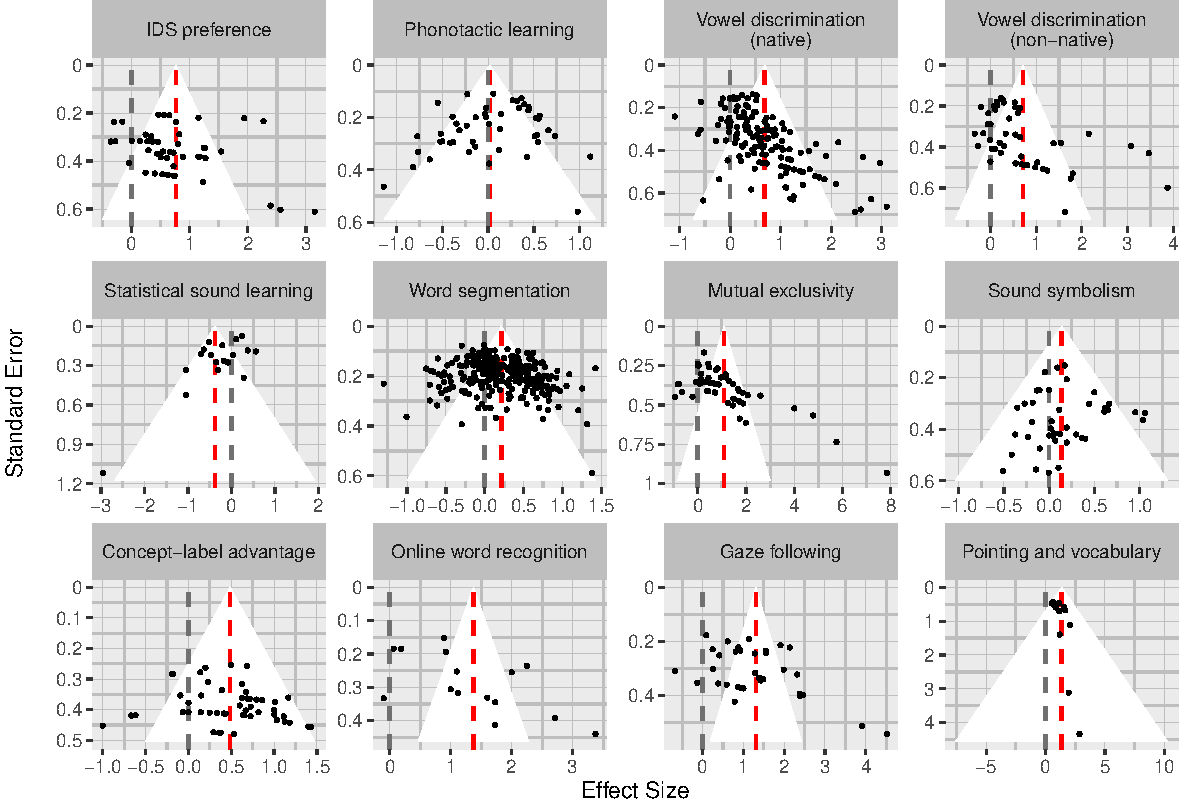
\includegraphics{metalab_synthesis_files/figure-latex/unnamed-chunk-2-1.pdf}
\caption{\label{fig:unnamed-chunk-2}Funnel plots for each meta-analysis.
Each effect size estimate is represented by a point, and the mean effect
size is shown as a red dashed line. The grey dashed line shows an effect
size of zero. The funnel corresponds to a 95\% CI around this mean. In
the absence of true heterogeneity in effect sizes (no moderators) and
bias, we should expect all points to fall inside the funnel.}
\end{figure}

Funnel plots provide a visual method for evaluating whether variability
in effect sizes is due only to differences in sample size. A funnel plot
shows effect sizes versus a metric of sample size, standard error. If
there is no bias in a literature, we should expect studies to be
randomly sampled around the mean, with more variability for less precise
studies. Figure 1 presents funnel plots for each of our 12
meta-analyses. These plots show evidence of asymmetry (bias) for several
of our phenomena (Table 2, column 4). An important limitation of this
method, however, is that it is difficult to determine the source of this
bias. One possibility is that this asymmetry reflects true heterogeneity
in phenomena affecting both effect size and precision (e.g., a test of
older infants may require fewer participants because their performance
is more stable and yields a larger
effect).\footnote{The role of moderators such as age can be interactively explored on the Metalab website (http://metalab.stanford.edu).}
P-curve analyses provide one method for addressing this issue, which we
turn to next.

\subsection{P-curves}\label{p-curves}

\begin{figure}
\centering
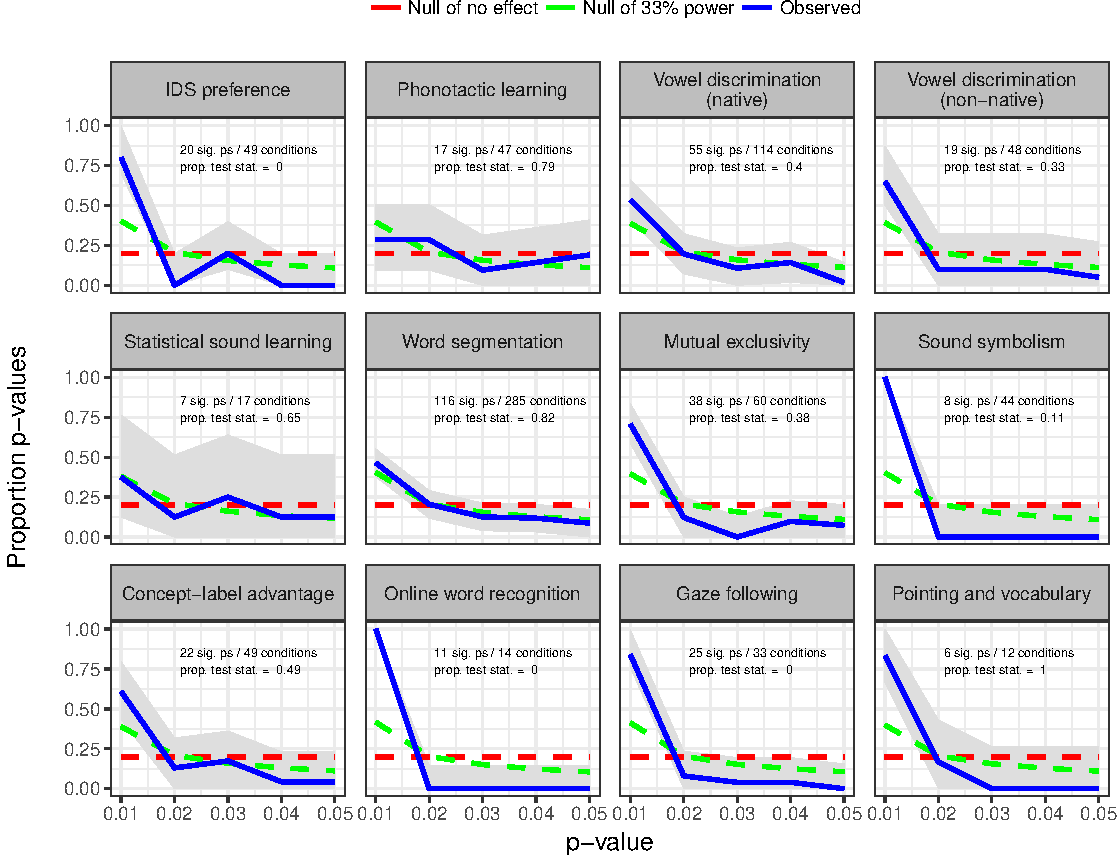
\includegraphics{metalab_synthesis_files/figure-latex/p_curve_plots-1.pdf}
\caption{(\#fig:p\_curve\_plots)P-curve for each meta-analysis
(Simonsohn, Nelson, \& Simmons, 2014). In the absence of p-hacking, we
should expect the observed p-curve (blue) to be right-skewed (more small
values). The red dashed line shows the expected distribution of p-values
when the effect is non-existent (the null is true). The green dashed
line shows the expected distribution if the effect is real, but studies
only have 33\% power. Grey ribbons show 95\% confidence intervals
estimated from a multinomial distribution. Text on each plot shows the
number of p-values for each dataset that are less than .05 and thus are
represented in each p-curve (\enquote{sig. ps}), relative to the total
number of conditions for that phenomenon. Each plot also shows the
proportion of p-values that were derived from test statistics reported
in the paper (\enquote{prop. test stat.}); all others were derived by
conducting analyses on the descriptive statistics or transforming
reported effect sizes.}
\end{figure}

A p-curve is the distribution of p-values for the statistical test of
the main hypothesis across a literature (Simonsohn et al., 2014b, 2014a,
2015). Critically, if there is a robust effect in the literature, the
shape of the p-curve should reflect this. In particular, we should
expect the p-curve to be right-skewed with more small values (e.g., .01)
than large values (e.g., .04). An important property of this analysis is
that that the should be skew independent of any true heterogeneity in
the data, such as age. Evidence that the curve is in fact right-skewed
would suggest that the literature is not biased, and that it provides
evidential value for theory building.

P-values for each condition were calculated based on the reported test
statistic. However, test statistics were not available for many
conditions, either because they were not reported or because they were
not coded. To remedy this, we also calculated p-values indirectly based
on descriptive statistics (means and standard deviations; see SI for
details).

Figure 2 shows p-curves for each of our 12 meta-analyses. All p-curves
show evidence of right skew, with the exception of phonotactic learning
and statistical sound learning (Table 2, column 5). This pattern did not
differ when only reported test-statistics were used to calculate
p-curves (see SI).

In sum, then, meta-analytic methods, along with our dataset of effect
sizes, provide an opportunity to assess the replicability of the field
of language acquisition. Across a range of analyses, we find that this
literature shows some evidence for bias, but overall, it is quite
robust.

\section{Quantitative Evaluation of
Theories}\label{quantitative-evaluation-of-theories}

Next, we turn to how these data can be used to constrain and develop
theories of language acquisition.

Meta-analytic methods provide a precise, quantitative description of the
developmental trajectory of individual phenomena. Figure 3 presents the
developmental trajectories of the phenomena in our dataset at each level
in the linguistic hierarchy. By describing how effect sizes change as a
function of age, we can begin to understand what factors might moderate
that trajectory, such as aspects of a child's experience or maturation.
For example, the meta-analysis on mutual exclusivity (the bias for
children to select a novel object, given a novel word; Markman \&
Wachtel, 1988) suggests a steep developmental trajectory of this skill.
We then can use these data to build quantitative models to understand
how aspects of experience (e.g., vocabulary development) or maturational
constraints may be related to this trajectory (e.g., Frank, Goodman, \&
Tenenbaum, 2009; McMurray, Horst, \& Samuelson, 2012).

In addition, meta-analytic methods provide an approach for synthesizing
across different linguistic skills via the common metric of effect
sizes. The ultimate goal is to use meta-analytic data to build a single,
quantitative model of the language acquisition system, much like those
developed for individual language acquisition phenomena, like word
learning. Developing a single quantitative model is a lofty goal,
however, and will likely require much more precise description of the
phenomena than is available in our dataset. Nevertheless, we can use our
data to distinguish between broad classes of theories about the
interdependency of skills.

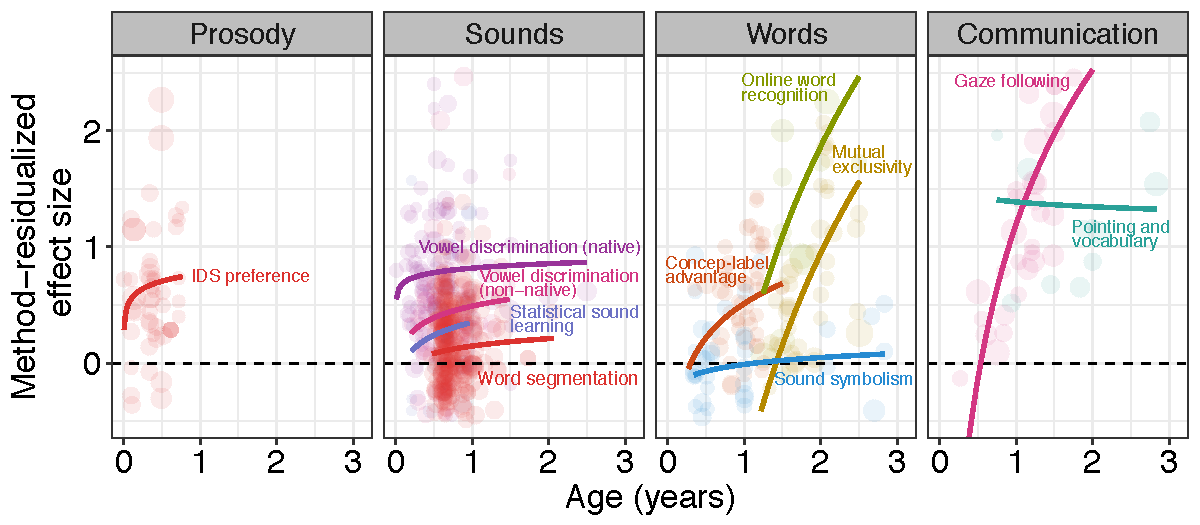
\includegraphics{figs/fig3_lab.pdf} We first consider two broad theories
of learning dependencies that have been articulated in a number of
forms, and which we will clearly separate for the purposes of
exposition. At one extreme, there is the stage-like theory which posits
that linguistic skills are acquired in a strictly sequential manner,
beginning with skills at the lowest level of the linguistic hierarchy
and working their way up. Under this theory, once a skill is mastered,
and only then, can it be used to support the acquisition of skills
higher in the linguistic hierarchy. In this way, a child sequentially
acquires the skills of language, \enquote{bootstrapping} from existing
knowledge at lower levels to new knowledge at higher levels. Consistent
with this theory, there is evidence that prosody supports the
acquisition of sound categories (e.g., Werker et al., 2007), word
boundaries (e.g., Jusczyk, Houston, \& Newsome, 1999), grammatical
categories (e.g., Shi, Werker, \& Morgan, 1999), and even word learning
(e.g., Shukla et al., 2011).

\begin{figure}
\centering
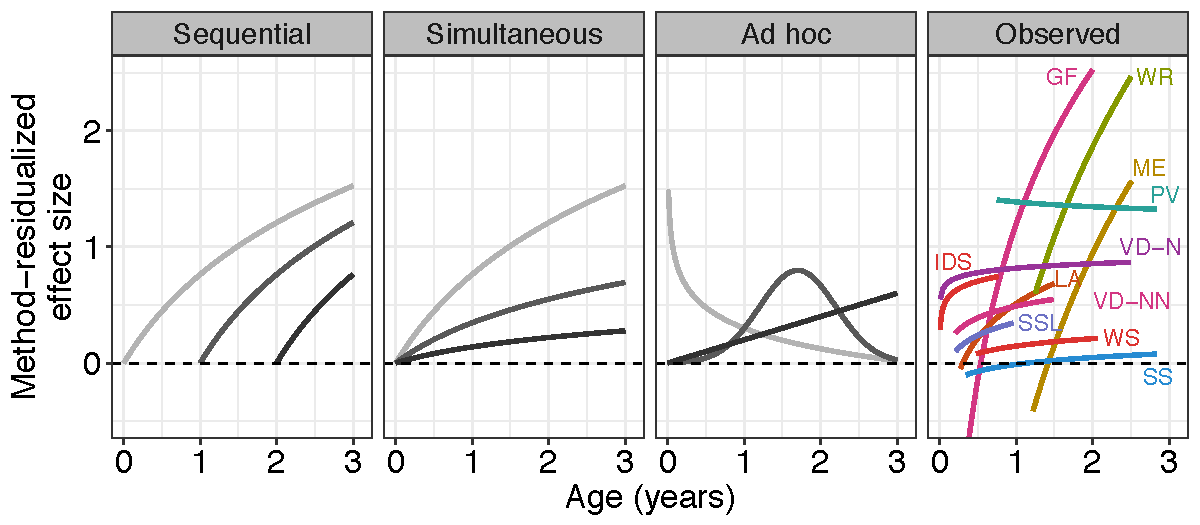
\includegraphics{figs/fig4_lab.pdf}
\caption{\label{fig:unnamed-chunk-6}The left two panels show the
developmental trajectories predicted under different meta-theories of
language acquisition. The stage-like theory predicts that a child will
not begin learning the next skill in the linguistic hierarchy until the
previous skill has been mastered. The interactive theory predicts that
multiple skills may be simultaneously acquired. The third panel shows
other possible developmental trajectories (decreasing, linear, and
non-monotonic). The fourth panel shows the observed meta-analytic data.
Effect size is plotted as a function of age from 0-3 years, across 10
different phenomena (excluding phonotactic learning and sound category
learning). Model fits are the same as in Figure 3. These developmental
curves suggest there is interactivity across language skills, rather
than stage-like learning of the linguistic hierarchy. GF: Gaze
following; IDS: IDS preference; LA: Concept -label advantage; ME: Mutual
exclusivity; VD-(N)N: Vowel discrimination (non-)native; PV:
Pointing-vocabulary correlations; SS: Sound symbolism; WR: Word
recognition.}
\end{figure}

Alternatively, multiple skills may be learned simultaneously across the
system regardless of their place in the hierarchy, and potentially with
top-down effects. There is evidence that higher-level skills like word
learning may be acquired relatively early in development, likely before
phonological learning has been completed (e.g., Bergelson \& Swingley,
2012; Tincoff \& Jusczyk, 1999). The possibility that higher levels may
be learned concurrently or even previous to lower levels is consistent
with predictions of a class of hierarchical Bayesian models that suggest
that more abstract knowledge may be acquired quickly, before lower-level
information, and may in turn support the acquisition of lower
information (``blessing of abstraction,'' Goodman, Ullman, \& Tenenbaum,
2011). There is evidence for this proposal from work that suggests word
learning supports the acquisition of lower-level information like
phonemes (Feldman et al., 2013).

These two theories make different predictions about relative
trajectories of skills across development. Within the meta-analytic
framework, we can represent these different trajectories schematically
by plotting the effect sizes for different skills across development. In
particular, the bottom-up theory predicts serial acquisition of skills
(Figure 4; left) while the interactive theory predicts simultaneous
acquisition (left center). We can also specify many other possible
trajectories by varying the functional form and parameters of the model.
Figure 4 (\enquote{Ad hoc}; right center) shows several other possible
trajectories. For example, a skill might have a non-monotonic
trajectory, increasing with age, and then decreasing. By specifying the
shape of these developmental trajectories and the age at which
acquisition begins, we can consider many patterns of developmental
trajectories, and how these different patterns, in turn, constrain our
meta-theories of development.

Our data allow us to begin to differentiate between this space of
theories. Figure 4 (right) presents a synthetic representation of the
developmental trajectories of the skills in our dataset with literatures
shown to have evidential value (all but phonotactic learning). We find
strong evidence for the simultaneous acquisition of skills---children
begin learning even high-level skills, like the meanings of words, early
in development, and even low-level skills like sound categories show a
protracted period of development. This pattern is less consistent with
stage-like theories than with parallel or top-down theories of language
acquisition. In future research, we can use this approach to distinguish
between a larger space of meta-theories and, ultimately, refine our way
towards a single quantitative theory of language acquisition.

\section{Discussion}\label{discussion}

Building a theory of a complex psychological phenomenon requires making
good inductive inferences from the available data. Meta-analysis can
support this process by providing a toolkit for quantitative description
of individual behaviors and their relationship to important moderators
(e.g., age, in our case). Here, we apply the meta-analytic toolkit to
the domain of language acquisition---a domain where there are concerns
of replicability, and where high-fidelity data are needed for theory
building. We find that the existing literature in this domain describes
mostly robust phenomena and thus should form the basis of theory
development. We then aggregate across phenomena to offer the first
quantitative synthesis of the field. We find evidence that linguistic
skills are acquired simultaneously rather than in a stage-like fashion.

In this paper, we focused on theoretical motivations for building
meta-analysis, but naturally, there are many other practical reasons for
conducting a quantitative synthesis. For example, when planning an
experiment, an estimate of the size of an effect on the basis of prior
literature can inform the sample size needed to achieve a desired level
of power. Meta-analytic estimates of effect sizes can also aid in design
choices: If a certain paradigm or measure tends to yield overall larger
effect sizes than another, the strategic researcher might select this
paradigm in order to maximize the power achieved with a given sample
size. These and other advantages, illustrated with the same database
used here, are explained in Bergmann et al.~(in press).

Despite its potential, there are a number of important limitations to
the meta-analytic method as tool for theory building in psychological
research. One challenging issue is that in many cases method and
phenomenon are confounded. This is problematic because a method with
less noise than another will produce a bigger effect size for the same
phenomenon. As a result, it is difficult to determine the extent to
which a difference in effect size between two phenomena is due to an
underlying difference in the phenomena, or merely to a difference in
they way it was tested. While method may account for some variability in
our dataset, we find that method does not have a large impact on effect
size for phenomena relative to other moderators like age (see SI).
Nevertheless, covariance between method and phenomenon, as found in our
dataset and probably many other fields of study, limits our ability to
directly compare effect sizes across phenomena.

Second, meta-analysis, like all analytical methods, requires the
researcher to make analytical decisions, and these decisions may be
subject to the biases of the researcher. We believe that a virtue of the
current approach is that we have applied the same analytical method
across all phenomena we examined, thus limiting our \enquote{degrees of
freedom} in the analysis. However, in some cases this uniform approach
to data analysis means that we are unable to take into consideration
aspects of a particular phenomenon that might be relevant. For example,
in a study using the vowel discrimination and word segmentation datasets
to adjudicate bottom-up versus top-down theories, Bergmann, Tsuji, and
Cristia (2017) concluded this was effectively studied only when
subsetting to papers that tested at least two different age groups as a
way of focusing on age differences while controlling for other possible
differences between experiments. Here, we have followed a different
route, by normalizing effect sizes across methods. We believe that the
systematic, uniform analytical approach used here is the most
appropriate for minimizing bias by the meta-analyst. Notably, this
analytical decision has consequences for interpretation: Bergmann,
Tsuji, and Cristia (2017) found a moderate decrease in effect size with
age for non-native vowel discrimination, while the current analysis
suggests a moderate increase. We thus recommend future researchers to
consider this question carefully, particularly in meta-analyses with
high heterogeneity.

While meta-analysis uniquely provides a high-level view of the empirical
landscape, we consider the meta-analytic method as synergistic with
other methodological approaches. Notably, one of the critical features
of a meta-theory of language acquisition is proposed causal relationship
between different skills. For example, the interactive theory suggests
that skills at higher levels \emph{support} the acquisition at lower
levels, even before skills at lower levels are mastered. In the
meta-analytic framework, this predicts that there should be simultaneous
development of skills across the language hierarchy---as we observe in
the current work. Importantly, however, this analysis is inherently
correlational, entailing that we cannot directly infer a causal
relationship between acquisition at lower levels and acquisition at
higher levels. That is, while the observed pattern is consistent with
the interactive theory, it is also possible that there is no causal
relationship between skills across the language hierarchy, merely
parallel trajectories of acquisition. For this reason, experimental work
must go hand-in-hand with meta-analysis to address causal questions.

Finally, there are a number of important limitations to the
meta-analytic method more broadly. One issue is that the method relies
on researchers conducting replications of the same study across a range
of ages and, critically, reporting these data so that they can be used
in meta-analyses. To the extent that researchers do not conduct these
studies, or report the necessary statistics in their write-ups (e.g.,
means and standard deviations), the meta-analytic method cannot be
applied. In addition, the meta-analytic method, as in the case of
qualitative forms of synthesis (e.g., literature review), is limited by
the potential presence of bias, which can come from a range of sources
including non-representative participant populations, failure to publish
null findings, and analytical degrees-of-freedom. To the extent these
biases are present in the literature, methods of synthesizing these
findings will also be biased. Nevertheless, meta-analytic methods for
aggregating even the smallest sample of studies are likely to be less
biased than qualitative methods (Valentine, Pigott, \& Rothstein, 2010).

In sum, understanding the psychological mechanisms underlying complex
phenomena is a difficult inferential task: The researcher must develop a
predictive and explanatory theory on the basis of limited and noisy
experimental data. Here we have focused on language acquisition as a
case study of how meta-analytic methods can be productively leveraged as
a tool for theory building. Meta-analytic methods allow the researcher
to determine whether phenomena are robust, synthesize across
contradictory findings, and ultimately, build an integrative theory
across phenomena. Moving forward, we see meta-analysis as a powerful
tool in the researcher's toolkit for developing quantitative theories to
account for complex psychological phenomena.

\section{Methods}\label{methods}

We analyzed 12 different phenomena in language acquisition. We selected
these particular phenomena because of their theoretical importance or
because a previously-published meta-analysis already existed.

To obtain estimates of effect size, we either coded or adapted others'
coding of papers reporting experimental data (see SI for details).
Within each paper, we calculated a separate effect size estimate for
each experiment and age group (we refer to each measurement separated by
age as a \enquote{condition}). In total, our sample includes estimates
from 232 papers, 777 different conditions and 13,988 participants. The
process for selecting papers from the literature differed by domain,
with some individual meta-analyses using more systematic approaches than
others (see SI for specific search strategies). Nevertheless,
meta-analytic methods for aggregating even the smallest sample of
studies are likely to be less biased than qualitative methods
(Valentine, Pigott, \& Rothstein, 2010).

sum(all\_data\$n\_1)

\paragraph{Data and Code Availability}\label{data-and-code-availability}

The data and code reported in this paper have been deposited in GitHub,
a web-based repository hosting service,
\url{https://github.com/langcog/metalab/}.

\paragraph{Supplementary Information}\label{supplementary-information}

This article contains supporting information online at
\url{http://rpubs.com/mll/synthesisSI}

\newpage

\subsubsection{References}\label{references}

\setlength{\parindent}{-0.5in} \setlength{\leftskip}{0.5in}
\setlength{\parskip}{8pt}

\hypertarget{refs}{}
\hypertarget{ref-anderson2016response}{}
Anderson, C. J., Bahník, Š., Barnett-Cowan, M., Bosco, F. A., Chandler,
J., Chartier, C. R., \ldots{} others. (2016). Response to comment on
``estimating the reproducibility of psychological science''.
\emph{Science}, \emph{351}(6277), 1037--1037.

\hypertarget{ref-bergelson2016}{}
Bergelson, E., \& Swingley, D. (2012). At 6--9 months, human infants
know the meanings of many common nouns. \emph{Proceedings of the
National Academy of Sciences}, \emph{109}(9), 3253--3258.

\hypertarget{ref-bergmann2015development}{}
Bergmann, C., \& Cristia, A. (2015). Development of infants'
segmentation of words from native speech: A meta-analytic approach.
\emph{Developmental Science}, \emph{19}(6), 901--917.

\hypertarget{ref-bergmann2017}{}
Bergmann, C., Tsuji, S., \& Cristia, A. (2017). Top-down versus
bottom-up theories of phonological acquisition: A big data approach. In
\emph{Proceedings of Interspeech 2017} (pp. 2013--2016).

\hypertarget{ref-bergmanneducational}{}
Bergmann, C., Tsuji, S., Piccinini, P., Lewis, M., Braginsky, M., Frank,
M., \& Cristia, A. (in press). Promoting replicability in developmental
research through meta-analyses: Insights from language acquisition
research. \emph{Child Development}.

\hypertarget{ref-button2013power}{}
Button, K. S., Ioannidis, J. P., Mokrysz, C., Nosek, B. A., Flint, J.,
Robinson, E. S., \& Munafò, M. R. (2013). Power failure: Why small
sample size undermines the reliability of neuroscience. \emph{Nature
Reviews Neuroscience}, \emph{14}(5), 365--376.

\hypertarget{ref-colonnesi2010relation}{}
Colonnesi, C., Stams, G. J. J., Koster, I., \& Noom, M. J. (2010). The
relation between pointing and language development: A meta-analysis.
\emph{Developmental Review}, \emph{30}(4), 352--366.

\hypertarget{ref-cristiastatisticalinprep}{}
Cristia, A. (in prep). Infants' phonology learning in the lab.

\hypertarget{ref-dunst2012preference}{}
Dunst, C., Gorman, E., \& Hamby, D. (2012). Preference for
infant-directed speech in preverbal young children. \emph{Center for
Early Literacy Learning}, \emph{5}(1).

\hypertarget{ref-ebersole2015many}{}
Ebersole, C., Atherton, O., Belanger, A., Skulborstad, H., Adams, R.,
Allen, J., \& Nosek, B. (2016). Many Labs 3: Evaluating participant pool
quality across the academic semester via replication. \emph{Journal of
Experimental Social Psychology}, \emph{67}, 68--82.

\hypertarget{ref-feldman2013word}{}
Feldman, N. H., Myers, E. B., White, K. S., Griffiths, T. L., \& Morgan,
J. L. (2013). Word-level information influences phonetic learning in
adults and infants. \emph{Cognition}, \emph{127}(3), 427--438.

\hypertarget{ref-frank2009using}{}
Frank, M., Goodman, N. D., \& Tenenbaum, J. B. (2009). Using speakers'
referential intentions to model early cross-situational word learning.
\emph{Psychological Science}, \emph{20}(5), 578--585.

\hypertarget{ref-frank2016performance}{}
Frank, M., Lewis, M., \& MacDonald, K. (2016). A performance model for
early word learning. In \emph{Proceedings of the 38th Annual Conference
of the Cognitive Science Society}.

\hypertarget{ref-Gilbert1037}{}
Gilbert, D. T., King, G., Pettigrew, S., \& Wilson, T. D. (2016).
Comment on Estimating the reproducibility of psychological science.
\emph{Science}, \emph{351}(6277), 1037--1037.
doi:\href{https://doi.org/10.1126/science.aad7243}{10.1126/science.aad7243}

\hypertarget{ref-glass1976primary}{}
Glass, G. V. (1976). Primary, secondary, and meta-analysis of research.
\emph{Educational Researcher}, \emph{5}(10), 3--8.

\hypertarget{ref-goodman2011learning}{}
Goodman, N. D., Ullman, T. D., \& Tenenbaum, J. B. (2011). Learning a
theory of causality. \emph{Psychological Review}, \emph{118}(1), 110.

\hypertarget{ref-hedges2014statistical}{}
Hedges, L. V., \& Olkin, I. (2014). \emph{Statistical methods for
meta-analysis}. Academic press.

\hypertarget{ref-johnson2010synergies}{}
Johnson, M., Demuth, K., Jones, B., \& Black, M. J. (2010). Synergies in
learning words and their referents. In \emph{Advances in neural
information processing systems} (pp. 1018--1026).

\hypertarget{ref-jusczyk1999beginnings}{}
Jusczyk, P. W., Houston, D. M., \& Newsome, M. (1999). The beginnings of
word segmentation in english-learning infants. \emph{Cognitive
Psychology}, \emph{39}(3), 159--207.

\hypertarget{ref-kuhl2004early}{}
Kuhl, P. K. (2004). Early language acquisition: Cracking the speech
code. \emph{Nature Reviews Neuroscience}, \emph{5}(11), 831--843.

\hypertarget{ref-lammertink2016}{}
Lammertink, I., Fort, M., Peperkamp, S., Fikkert, P., Guevara-Rukoz, A.,
\& Tsuji, S. (2016). SymBuki: A meta-analysis on the sound-symbolic
bouba-kiki effect in infants and toddlers. Poster presented at the XXI
Biennial International Congress of Infant Studies, New Orleans, USA.

\hypertarget{ref-lfprep}{}
Lewis, M. L., \& Frank, M. (in prep). Mutual exclusivity: A
meta-analysis.

\hypertarget{ref-lewisunpublished}{}
Lewis, M., \& Long, B. (unpublished). Meta-analysis of the concept-label
advantage.

\hypertarget{ref-markman1988}{}
Markman, E., \& Wachtel, G. (1988). Children's use of mutual exclusivity
to constrain the meanings of words. \emph{Cognitive Psychology},
\emph{20}(2), 121--157.

\hypertarget{ref-mcmurray2012word}{}
McMurray, B., Horst, J. S., \& Samuelson, L. K. (2012). Word learning
emerges from the interaction of online referent selection and slow
associative learning. \emph{Psychological Review}, \emph{119}(4), 831.

\hypertarget{ref-open2012open}{}
Open Science Collaboration. (2012). An open, large-scale, collaborative
effort to estimate the reproducibility of psychological science.
\emph{Perspectives on Psychological Science}, \emph{7}(6), 657--660.

\hypertarget{ref-open2015estimating}{}
Open Science Collaboration. (2015). Estimating the reproducibility of
psychological science. \emph{Science}, \emph{349}(6251), aac4716.

\hypertarget{ref-orwin1983fail}{}
Orwin, R. G. (1983). A fail-safe N for effect size in meta-analysis.
\emph{Journal of Educational Statistics}, 157--159.

\hypertarget{ref-scargle1999publication}{}
Scargle, J. D. (2000). Publication bias: The ``file-drawer problem'' in
scientific inference. \emph{Journal of Scientific Exploration},
\emph{14}(1), 91--106.

\hypertarget{ref-shi1999newborn}{}
Shi, R., Werker, J. F., \& Morgan, J. L. (1999). Newborn infants'
sensitivity to perceptual cues to lexical and grammatical words.
\emph{Cognition}, \emph{72}(2), B11--B21.

\hypertarget{ref-shukla2011prosody}{}
Shukla, M., White, K. S., \& Aslin, R. N. (2011). Prosody guides the
rapid mapping of auditory word forms onto visual objects in 6-mo-old
infants. \emph{Proceedings of the National Academy of Sciences},
\emph{108}(15), 6038--6043.

\hypertarget{ref-simonsohn2014power}{}
Simonsohn, Nelson, L. D., \& Simmons, J. P. (2014a). P-curve and effect
size correcting for publication bias using only significant results.
\emph{Perspectives on Psychological Science}, \emph{9}(6), 666--681.

\hypertarget{ref-simonsohn2014p}{}
Simonsohn, Nelson, L. D., \& Simmons, J. P. (2014b). P-curve: A key to
the file-drawer. \emph{Journal of Experimental Psychology: General},
\emph{143}(2), 534.

\hypertarget{ref-simonsohn2015better}{}
Simonsohn, Simmons, J. P., \& Nelson, L. D. (2015). Better p-curves.
\emph{Journal of Experimental Psychology: General}, \emph{144}(6),
1146--52.

\hypertarget{ref-sterne2005regression}{}
Sterne, J. A., \& Egger, M. (2005). Regression methods to detect
publication and other bias in meta-analysis. \emph{Publication Bias in
Meta-Analysis: Prevention, Assessment, and Adjustments}, 99--110.

\hypertarget{ref-tincoff1999some}{}
Tincoff, R., \& Jusczyk, P. W. (1999). Some beginnings of word
comprehension in 6-month-olds. \emph{Psychological Science},
\emph{10}(2), 172--175.

\hypertarget{ref-valentine2010many}{}
Valentine, J. C., Pigott, T. D., \& Rothstein, H. R. (2010). How many
studies do you need? A primer on statistical power for meta-analysis.
\emph{Journal of Educational and Behavioral Statistics}, \emph{35}(2),
215--247.

\hypertarget{ref-werker2007infant}{}
Werker, J. F., Pons, F., Dietrich, C., Kajikawa, S., Fais, L., \& Amano,
S. (2007). Infant-directed speech supports phonetic category learning in
English and Japanese. \emph{Cognition}, \emph{103}(1), 147--162.






\end{document}
